\section{Background and Introduction}
\label{sec:intro}  

\section*{Introduction: A reconfigurable reinforcement learning method}

\subsection{Paper outline} \circled{$\alpha$} General RL-mapping prior knowledge ($\tilde{R}$ and $\tilde{T}\to\tilde{Q}$)\\

\subsubsection{Introduction} 

One of the largest issues facing Q-Learning and Reinforcement Learning is the coupling of reward and state behaviours. In humans, this behaviour is called anchoring. A person can learn to associate reward with stimulus via Pavlov's effect. Importantly, humans possess the ability to disassociate reward from the prediction of system dynamics. For robots to be truly flexible learners, they must be able to separately encode the reward in a system from the transition dynamics in a system.  This allows one robot to maximize different reward functions without retraining.

\subsubsection{Q-Learning Extension}

Specifically, given a perfect encoding $Q^\ast(s, a)$, transition and reward are 
\begin{equation}
\argmax_{a} Q_t^\ast(s,a)\sim\pi^\ast(s) = \argmax_{a} \sum_{s^\prime} R( s^\prime | a, s ) T( s^\prime | a, s ) + \gamma V( s^\prime )
\end{equation}
where
\begin{align}
Q^\ast_t(s,a) & = Q_{t-1}(s,a)+\alpha \left( Q_{t-1}( s, a ) - R( s^\prime | s, a ) \right) + \gamma Q_{t-1} ( s^\ast, a^\ast ) \\
Q^\ast_t(s,a) & = Q_{t-1}(s,a)+\alpha \left( Q_{t-1}( s, a ) - R( s^\prime | s, a ) \right) + \gamma \argmax_{a^\ast} Q ( s^\prime, a^\ast )
\end{align}
Unfortunately, as time $t$ increases in value, the values $R(s|s)$ and $T(s|a,s)$ are encoded such that $f:R\cdot T\to Q_0$ it is not possible to compute $f^{-1}(Q)$ due to the loss of information. 

To avoid information loss, a dynamics equation $\tilde{T}$ and observed reward policy $\tilde{R}$ can be tracked, and used to compute at any
 time:
\begin{equation}
\tilde{Q}^\ast_t( s, a ) = \sum_{s^\prime} \tilde{T}_{t-1}^\ast ( s^\prime | s, a ) \tilde{R}_{t-1}( s^\prime, s, a ) + \gamma \pi^\ast( s^\prime ) \label{eq:a.2} 
\end{equation}
where $\tilde{\pi}^\ast( s, a ) \sim Q^\ast( s, a )$. 

It is clear that (\ref{eq:a.2}) must iterate over all states $s^\prime$, which is intractable. However, if optimal policy locality for a function $L$ is assumed, the resulting expression~\ref{eq:} is optimal.

\underline{Lemma 1}: Policy optimality for the purposes of regresssion to optimal Q values $(\tilde{Q}^\ast, Q^\ast )$, consideration of ``local'' states and ``local'' acting are required,
\begin{equation}
L:S,A\to S,A | \text{onto}
\end{equation}
\begin{equation}
\sum_{S^\prime \in S} \tilde{T}_t ( s^\prime | s, a ) \tilde{R}_t( s^\prime | s, a ) +\gamma \tilde{\pi}( s^\prime )  = \sum_{S \in L(s)}  \tilde{T}_{t}( s^\prime | s, a ) \tilde{R}_t( s^\prime | s, a ) + \tilde{\gamma}( s^\prime )
\end{equation}
\begin{equation}
\argmax_{a \in A}\tilde{Q}^\ast( s, a ) = \argmax_{a\in L(a)} \tilde{Q}^\ast( s, a )
\end{equation}
\begin{equation}
\tilde{\pi}^\ast( s | L ) = \tilde{\pi}^\ast( s )
\end{equation}
The local policy is equivalent to the complete state $\times$ action space version.\\

\subsubsection{Regression} 

Instead of regressing to Q values directly $\left( Q_t \leftarrow f(Q_{t-1}) \right)$ we instead regress to system dynamics $\left( \tilde{T}_t \leftarrow f( T_{t-1} ) \right)$. Specifically:
\begin{align}
\tilde{T}_{t+1}( s^\prime | s, a ) = \frac{\textit{freqn}(s^\prime | s, a )}{\textit{freqn}( s, a )} & \quad\text{or}\quad \tilde{T}_{t+1}( s^\prime | s, a ) = P( s^\prime | s, a ) \\
\underbrace{\tilde{R}_{t+1}( s^\prime | s, a ) = R_t( s^\prime | s, a )}_{\text{simple}} & \quad\text{or}\quad \underbrace{\tilde{R}_{t+1}( s^\prime | s, a ) = \tilde{R}( s^\prime | s, a ) + \left( \tilde{R}( s^\prime | s, a ) - R( s^\prime, a, s ) \right)}_{\text{verbose}} 
\end{align}
\textasteriskcentered --- $\tilde{T} \approx T$ when

Thus it is possible, using either a simple regression model or a verbose training model, to regress to an optimal policy $\tilde{\pi}^\ast$, online, and exploit reward switching.

\subsubsection{Behaviour Switching}

After an agent is trained ($\tilde{\pi}\sim\tilde{\pi}^\ast$), then it is possible to redefine the reward function $\tilde{R}$. Given $\tilde{R}_{t} = R_{A}$, then $\tilde{R}_{t+1} \leftarrow R_{B}$ is possible. At this point the transition dynamics ($\tilde{T}$) and locality principle ($L$) maybe be used to infer $\tilde{\pi}_{t+1}$. Just as a human may redefine an objective during learning, agents may also change the definition of success through reassignment of $\tilde{R}$.

\paragraph{Optimality of Switching}

Given a set of reward functions $\mathbf{R}=\{R_1, R_2, \ldots \}$ and a set of time indexes $\{ 1, 2, 3, \ldots, t, \ldots \}$ as time approaches infinity ($t \to \infty$) the global policy $\tilde{\pi}^\ast_{t}(s)$ will converge on the optimal policy $\tilde{\pi}^\ast$, $\tilde{\pi}^\ast \in \Pi(R_i)$, where $\Pi(R_i)$ is the set of all optimal policies for reward function $R_i$.


Set of reward functions characterizing a set of goals
\begin{equation}
\mathbf{R}=\left\{ R_1, R_2, \ldots, R_i, \ldots \right\}\qquad R_i: S \times A \times S  = \mathbb{R}^{+}\,, \quad R_i\:\text{known} \leftarrow \mathbb{R}^{+}
\end{equation}
An ``expected quality'' of a state-action pair given locality \& states.
\begin{equation}
\tilde{Q}_t( s, a | R_i, L ) = \sum_{s^\prime \in L( s )} \tilde{T}_t( s^\prime | s, a) R( s^\prime | s, a ) + \gamma \argmax_{a^{*}} \tilde{Q}_{t}( s^\prime, a^\ast | R_i, L )
\end{equation}
Set of optimal policies
\begin{equation}
\Pi\,,\quad \pi^{*} \in \Pi \text{\ iif}: \pi^{\ast}( s ) = \argmax_{a} Q^{\ast}( s^\prime, a^{\ast} | L, R_i )
\end{equation}
optimal Q-value
\begin{equation}
Q^{\ast}( s, a | L, R_i  ) = \sum_{s^\prime \in L( s )} T( s^{\prime} | s, a ) R_i( s^\prime | s, a ) + \gamma \argmax_{a^{\ast}} Q^{\ast}
\end{equation}

1.\\
\begin{equation}
Q^{\ast}( s, a | L, R_i ) = \tilde{Q}_t( s, a | L, R_i )\,,\quad t \to \infty
\end{equation}
\begin{align}
Q^{\ast}( s, a | L, R_i ) & = E\left[ \sum_{s^{\prime} \in L( s )} T( s^{\prime} | s, a ) R_i( s^{\prime} | s, a ) + \gamma \argmax_{a^{\ast}} Q^{\ast}( s^{\prime}, a^{\ast} | R_i, L ) \right] \\
& = \sum_{s^{\prime} \in L( s )} E\left[ T( s^{\prime} | s, a ) \right] E\left[ R_i( s^{\prime} | s, a ) \right] + \gamma \argmax_{a^{\ast}} E\left[ Q^{\ast}( s^{\prime}, a^{\ast} | R_i, L ) \right] \\
& \qquad \qquad \qquad \text{obvious:\ }E[ Q^{\ast} ] \equiv Q^{\ast} \nonumber \\
& \qquad \qquad \qquad \text{obvious:\ }R_i( s^{\prime} | s, a ) \equiv E\left[ R_i( s^{\prime} | s, a ) \right] \nonumber \\
& = \sum_{s^{\prime} \in L(s)} E\left[ T( s^{\prime} | s, a ) \right] R_i( s^{\prime} | s, a ) + \gamma \argmax_{a^{\prime}} Q^{\ast}( s^{\prime}, a^{\ast} | R_i, L ) \\
\ast\:\text{Prove}\:\longrightarrow & \qquad \qquad \text{assert}\:\lim_{t \to \infty} \tilde{T}_t( s^{\prime} | s, a ) = E\left[ T( s^{\prime} | s, a ) \right] \nonumber \\
& = \lim_{t \to \infty} \sum_{s^{\prime} \in L( s )} \tilde{T}_t( s^\prime | s, a ) R_i( s^\prime | s, a ) + \gamma \argmax_{a^{\ast}} Q^{\ast}( s^{\prime}, a | R_i, L )
\end{align}
\begin{equation}
Q^{\ast}( s, a | L, R_i ) = \tilde{Q}_{t}( s, a | L, R_i )\,,\quad t \to \infty
\end{equation}
2.\\
Trivially: 
\begin{equation}
\text{if\ }\tilde{Q}_{t}( s, a | L, R_i ) \sim Q^{\ast}( s, a | L, R_i ) \text{\ iif\ }\tilde{T}_t \sim T
\end{equation}
\begin{equation}
\forall R_j \in \Pi: \tilde{Q}_t( s, a | L, R_j) \sim Q^{\ast}( s, a, L, R_j )
\end{equation}

\subsubsection{Validation}
To the value the efficiency of this model we consider a staged experiment with three reward functions.

Thus, in this experiment we consider training a model, first, on rewarding trading actions that essentially reward low exposure and no loss ($R_1$). Duriing this period $\tilde{T}$ will mature, and many dynamics of the system are discovered. After gains reach 10\%, $R_2$ becomes active --- given short term success in a security, we increase buy in. After this, given success, we reward an agent that tries to go ``all in'' to grow profits to 50\%. Lastly, at 50\%, we ``clamp'' the agent from being rewarded for taking excessive risks.

This reward profile, across industry, is common. Humans design reward profits and procedures that emphasize the result of behaviour. For example, on the trading floor, we are interested in policies that manage the risk--profit profile.

To experiment, we compose two processes:
\begin{enumerate}[label=\circled{\arabic*}]
\item a Q-learning mechanism
\item a $\tilde{T}$-learning mechanism
\end{enumerate}
For both models, the following definitions are used.\\

$S$ --- exposure $\times$ profit $\times$ price,$\qquad$ where exposure $\in [0,100]$, profit $\in \mathbb{R}$, price $\left\{ x\in \mathbb{R}^{+} \right\}_{x=0}^{100}$, representing exposure \%, profit \%, and price history \\

$A$ --- buy 1\%, sell 1\%, no action \\

$T$ --- $T( s^{\prime} | s, a )$ --- probability of making an action and ending up in a later state \\

$R$ --- \begin{equation}
R( s^{\prime} | s, a ) = \left\{ 
\begin{array}{ll}
R_1 \text{\ iif profit \textless 10\%} & R_1 = \frac{\Delta\text{profit}}{\text{exposure}}-\text{exposure} \\
R_2 \text{\ iif profit 10\% -- 20\%} & R_2 = \Delta\text{profit} \\
R_3 \text{\ iif profit 20\% -- 50\%} & R_3 = \Delta\text{profit(exposure)} \\
R_4 \text{\ iif profit 50\%+} & R_4 = \frac{\text{profit}}{\text{exposure}}
\end{array}
\right.
\end{equation}
$\tilde{T}$ --- predicted transitional dynamics --- encoded using random forrest classification \\

\begin{tabular}{|p{5cm}|p{3cm}|p{5cm}|}
Approach \circled{1} -- & Approach \circled{3} --  & Approach \circled{2} -- \\
Q-Learning & ensemble & T-learning \\
\hline
$R( s^\prime | s, a )$ will exhibit a `steady stochastic' 
 input pattern and the average reward $E[R(s^\prime|s,a)]$ 
will be encoded into the $Q(s,a)$ 
& 
We train separate Q-learning agents, each  which are active given the use of $R_1$, $R_2$, $R_3$, $R_4$, such that $R_i\to Q^{i}$.
& 
$\tilde{Q}(s,a)$ will never encode more than one, 
singular, reward function $R_t\approx\{ R_1, R_2, R_3, R_4 \}$.
Thus it is expected that T-learning will vastly out-perform Q-learning.
\end{tabular}

\subsubsection{Experiment}

We ran standard basic testing on two independent stocks.  One Google Inc., and the other, Blockbuster. Below we have plotted each models: Reward over time (Figure~\ref{}), Profit over time (Figure~\ref{}), Risk over time (Figure~\ref{}). All of the models are too juvenile in approach to be profitable. T-learning exhibits a xx\% increase in reward acquisition, a xx\% increase in profit and a xx\% increase in Reward. The ensemble approach failed to outperform the T-learning approach. The highest performance approach is T-learning.

\subsubsection{Summary}

In this paper a method of reusing experience over several reward functions was demonstrated. T-learning allows agents to recycle transtiion information discovered through online learning. The results of using this experiment in the financial domain was a reduction in model complexity, and increased performance. Using a singular Q-learning agent leads to a loss of understanding of the reward function. Using the ensemble approach requires the transition dynamics of the experiment to be encoded four times. Thus, T-learning had both the best performance, and can scale to an unlimited set of reward functions, without retraining. It is the opinion of the author that the encoding of transition and reward information separately should be seen as the fundamental first step when considering model reuse and generalization.


\subsection{RLN MDP structure}
\label{sec:rlnmdpstructure}

The general approach that is taken to form an RLN is ``split'' one single MDP into parent and child processes. Doing so assumes the two process are partly independent [CMDP]. 

\begin{enumerate}[label=\arabic*.]
\item Largely, the models may be independent.
\item The child and parent may include elements of each other's MDP definition in their own definition.
\end{enumerate}

This section focuses on framing a model. In Sections~\ref{sec:mapping} and later, subjects related to behavior optimality, convergence, and computational complexity are considered.

In order to consider the formation of a reconfigurable reinforcement network, it is required to analytically group all aspects of a process and a behavior policy into one tuples.

\begin{center}
\scalebox{0.5}{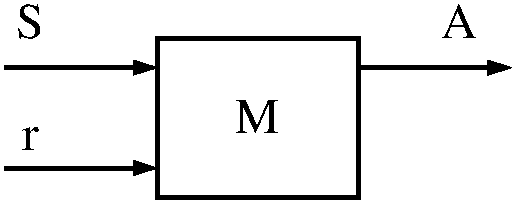
\includegraphics{media/page4diagram.pdf}}
\end{center}

To do this, assume a Markov decision process M which can be internally modeled as a tuple \( M = \langle S, A, T, R, \pi, \tilde{T}, \tilde{R}\rangle \)\\

$S$ -- a set of states $s\in S$ which may be experienced by $M$\\
$A$ -- a set of actions $a\in A$ that may be executed\\
$T$ -- a true transitional probability, $T(s^{\prime}|a,s)$ expressing the probability of executing an action $a$ in state $s$ before ending up in later state $s^{\prime}$.\\
$R$ -- is a reward function which quantifies how desirable a transition $R(s'|a,s)$ is. $R: S\times A \times S\rightarrow \mathbb{R}_{\geq 0}$\\
$\tilde{T}$ -- is the current model of $T$. The goal of $\tilde{T}$ is thus $\tilde{T}\sim T$\\
$\tilde{R}$ -- is the predicted reward of the system, constructed from observation of $R$, s.t.\ $\tilde{R}\rightarrow R$. \\
$\pi$ -- is an action selection policy, ideally chosen to maximize expected reward, an optimal policy is denoted $\pi^*$. Ideally
\begin{equation*}
\pi^*(s) = \argmax_{a}\sum_{s^\prime}\underbrace{R(s^\prime|a,s) T(s'|a,s)+\gamma V(s^\prime)}_{\text{expected reward}}
\end{equation*}
and
\begin{equation*}
\tilde{\pi}(s)  = \argmax_{a}\sum_{s^\prime}\tilde{R}(s^\prime|a,s) \tilde{T}(s'|a,s)+\gamma \tilde{V}(s^\prime)
\end{equation*}

\textbf{[Note that $\tilde{V}$ hasn't been defined in the previous equation.]}

\section*{encoding}

\begin{equation*}
\pi^*(s) = \argmax_{a}\sum_{s^\prime} R(s^\prime|s,a) T(s'|s,a)+\gamma V(s^\prime)
\end{equation*}
where
\begin{equation*}
V(s) = \sum_{s^\prime} R(s^\prime|s,a) T(s^\prime|s,a) +V(s^\prime)\,.
\end{equation*}
A bellman backup can be used [Bellman backup]. In online applications stochastic gradient descent can be applied to regress to locally optimal solutions. This allows estimation of optimal policy
\begin{equation*}
\pi^*(s) = \argmax_{a} Q(s,a)\,.
\end{equation*}

To encode the expected reward over all states, typically $Q$-values are kept: $ Q(s,a) \sim \sum R(s^\prime|a,s)T(s^\prime|a,s)+\gamma V(s^\prime) $ and $ Q_{t+1}(s,a) \leftarrow Q_t(s,a)+\alpha \left( R(s^\prime|a,s)-Q_t(s,a)+\gamma\argmax_{a^\prime} Q(s^\prime,a^\prime) \right) $.

To render the process $M$ separable, it is necessary to decouple the transitional values $T$ from the reward values $R$. Thus, to directly encode $Q(s,a)$ using $\pi$ is prohibitive.\\
knowing: 
\begin{equation*}
Q: S \times A \to \mathbb{R}_{\geq 0}
\end{equation*}
indirect encoding:
\begin{equation*}
\pi: \left\{ S \times A \times S \times \mathbb{N} \middle| R \right\} \to Q
\end{equation*}
If the definitions of $S$ or $A$ change, then $Q$ must be reinitialized. Alternatively, $\tilde{T}$ and $\tilde{R}$ are defined as intermediate encoding functions. Thus we define
\begin{equation*}
\pi:\left\{S \times A \times S \times \mathbb{N}\right\} \to \tilde{T}, \tilde{R}, Q
\end{equation*} 
simple transition
\begin{equation*}
\tilde{T}_{t+1}(s^\prime|s,a) = \frac{\textrm{freq}(s^\prime|s,a)}{\textrm{freq}(s,a)}
\end{equation*}
simple reward
\begin{equation*}
\tilde{R}_{t+1}(s^\prime|s,a) = \tilde{R}(s^\prime|s,a)+\alpha_R\left( \tilde{R}(s^\prime|s,a)-R(s^\prime|s,a)\right)
\end{equation*}
\begin{equation*}
f_Q: \tilde{T}_t \times \tilde{R}_t \to Q_t
\end{equation*}
In this paper we rely on a method of extracting dynamic $Q$-values from an encoded transition and reward function $( \tilde{T}, \tilde{R} )$. The motivation for this encoding is that it allows mapping the transition function into multiple spaces, and allows the reward function to be altered. The significance of this finding is covered in \textbf{???} Price wash \textbf{???}.

  
\subsection{Reconfiguration of $M$}

Reconfiguring a process $M$ allows some intractable MDPs to be rendered tractable. 
As an example, take an MDP $M$ modeling a 3-dimensional foraging experiment with three thousand positions on the $x$, $y$, and $z$
axes respectively. This process will consume over three billion memory locations and may be impossible to explore. If this system is
broken into three sub problems, each targeting a special axis, then only nine thousand memory locations need be consumed. This decreases memory requirements by an exponential factor.

This section presents a method of decomposition that, when followed, introduces no degeneration of the regressed policy $\pi^{*}(s,a)$.
The summary of these conditions is presented. There is no free lunch: the trade-off for saving in space is exponentially increased computational burden. As in all problems, finding the balance between space and computational complexity is required.

 

\subsubsection{Introduction to approach}

The general approach is related to factor analysis, or clustering, eigenvalue decomposition, or projected component analysis, with which the reader may be familiar. The process is split such that a subspace $S_i \subseteq S$, and action space $A_i \subseteq A$ seem independent of subspaces $S_k$, $A_k$, for the purposes of generating reward $R(s^\prime|a,s)$. Specifically, it may be observed that the reward is homogeneous, such that 
\begin{equation*}
\forall k_2, a_2: R\left(S^\prime_i \cup  S^\prime_{k_1} \middle| S_i \cup S_{k_1} , a_i \cup a_{k_1} \right) \sim R\left( S^\prime_i \cup S^\prime_{k_2}  \middle|  S_i \cup S_{k_2} , a_i \cup a_{k_2}  \right)\,.
\end{equation*}
In this case, it is likely that the problem may be separated. Even in the case where variance of reward is high, convergence is expected.

Splitting is done using a decomposition function
\begin{equation*}
d^{M_i,M_k}_{M} = M \longrightarrow \left\{    M_i, M_k \middle|
\begin{array}{l}
S_i \times ( S_k / \{s_i\} ) = S, S_k \times ( S_i / \{ s_k \} ) = S \\
A=A_i \cup A_k\\
\tilde{T}\sim d^{-1}(d(\tilde{T})),d(\tilde{T})=\tilde{T}_i, \tilde{T}_k\\
\tilde{R}\sim d^{-1}(d(\tilde{R})), d(\tilde{R})=\tilde{R}_i,\tilde{R}_k
\end{array}
 \right\}
\end{equation*}
where $d$ represents belief mapping functions that decompose and recompose $\tilde{T}$ and $\tilde{R}$. This allows  $M$ to be mapped as new spaces and observations are encountered. The decomposition process breaks one MDP into a parent and child:\\

\begin{center}
\scalebox{0.5}{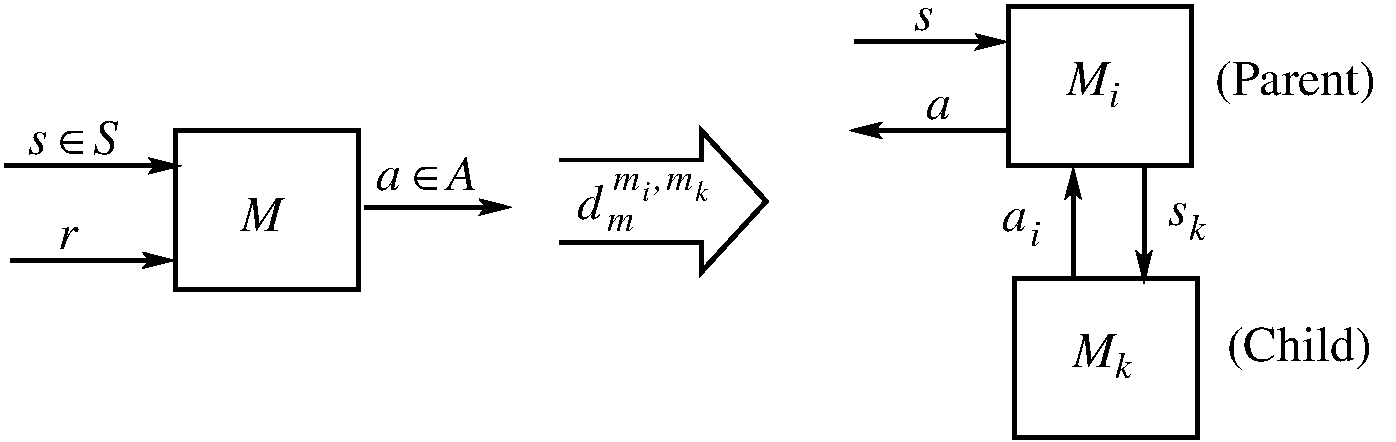
\includegraphics{media/page5figure}}
\end{center}


\newpage


Although many decomposition strategies are possible, this work presents a specific approach related to parent--child decomposition. This specific decomposition allows for assured policy convergence (see Section~\ref{})

\underline{Definitions}\\

\underline{$M$}\quad
\begin{minipage}[t]{5in}
$S=(S_i/S_k)\times(S_k/S_i)$\\
$A=A_i\cup A_k$\\
$T=P(S\times A\times S)$\\
$R= \text{real, positive, convergent stochastic as $t\to\infty$}$\\
$R(s^\prime,a,s) =R\left( 
\begin{array}{c} s^\prime_i \\ s^\prime_k \end{array},
\begin{array}{c} a_i \\ a_k \end{array},
\begin{array}{c} s_i \\ s_k \end{array}
\right)$
\end{minipage}\\

The system can be broken into the following MDP definitions

\underline{$M_i$ -- Parent}\\

$S_i$ -- a collection of states, $s_i\in S_i$\\
$A_i$ -- a collection of actions, $a_i \in A_i$\\
$\tilde{T}( s^\prime_i | s_i, a_i )$ -- the observed probability of executing action $a_i$ in state $s_i$ and ending up in state $s^\prime_i$\\

\begin{equation*}
\left. \begin{array}{l}
\tilde{T}\\
\tilde{R}
\end{array}\right\}
\text{Covered Pages on BII p12-14}
\end{equation*}

$P(s^\prime_i|s_i, a_i)$ is observed directly and is $\tilde{T}( s^\prime_i | s_i, a_i )$\\

%$R_t\left({}^{s^\prime_i}_{a^\prime_k}|{}_{a_i},{}^{s_i}_{a_k}\right)=R_t\left({}^{s^\prime_i}_{s^\prime_k},{}^{a_i}_{a_k},{}^{s_i}_{s_k}\right)$

\begin{equation*}
\tilde{R}_t\left(  \begin{array}{l} s^\prime_i \\ a^\prime_k \end{array}
\middle| 
\begin{array}{c}  a_i \\ \end{array},
\begin{array}{c} s_i \\ a_k \end{array}
\right) 
=
\tilde{R}_t\left( 
\begin{array}{c} s^\prime_i \\ s^\prime_k \end{array}, \middle|
\begin{array}{c} a_i \\ a_k \end{array},
\begin{array}{c} s_i \\ s_k \end{array}
\right)
=
\tilde{R}( s^\prime | a, s )
\end{equation*}


$S$, $T_i$, $S_k$, $S^\prime_k$ are not directly observable by process $M_i$, by design. Importantly, some facts are known about $a_k$ and $a^\prime_k$ which will be exploited in Section~\ref{}.\\

ii) $a_k=\pi_k(s_k)$\\
iii) $a^\prime_k=\pi_k(s_k)$\\
iiii) $\left(s_k,s^\prime_k\right)$ chosen indirectly by $\pi_k(\cdot)$ in a manner that assuming monotonic increase in reward,
\begin{equation*}
  \text{as\ }t \to \infty \quad E[R_{t+1}(\cdot)] \geq E[R_t(\cdot)]\,.
\end{equation*}
Local convergence of this process on a behavior policy $\pi^*_i(\cdot)$ is assured.

\underline{$M_k$ -- child}\\

$S^\prime_i$ -- all child states, $s_k\in S_k$\\
$a_k\in A_k$\\
$\tilde{T}(s^\prime_k|s_k,a_k)$\\
$R_t(s^\prime_k,a_k,s_k)=R_t\left({}^{s_i}_{s^\prime_k},{}^{a_i}_{a_k},{}^{s_i}_{s_k}\right)$
s.t.\ $s_i$, $s^\prime_i$ are chosen by another process, and
\begin{equation*}
\boxed{A^*}\quad\longrightarrow\quad E[R_{t+1}(\cdot)]\geq E[R_t(\cdot)]
\end{equation*}
It is direct to note that both processes $M_i$ and $M_k$ are guaranteed to converge on locally optimal policies $\pi_i(\cdot)$, $\pi_k(\cdot)$ as the limit of time approaches infinity. 

In following sections next steps are discussed:
\begin{itemize}
\item $\pi^\ast_i \times \pi^\ast_k \to \pi^\ast${\ }utilizing the degenerate-optimal policies (Section~\ref{})
\item $d^{M_i, M_k}_{M}$ -- how to map values while preserving information, avoiding degeneracies (Section~\ref{sec:mapping})
\end{itemize}

